\documentclass[11pt]{amsart}
\usepackage{amsmath,amsfonts,amssymb,amsthm,verbatim,multirow,url,subfig,footnote,graphicx,array,xr,booktabs,placeins,float}
\usepackage[usenames,dvipsnames]{color}
%  \usepackage[style=numeric,
%  doi=false,
%  isbn=false,
%  url=false]{biblatex}
\usepackage[utf8]{inputenc}
\usepackage[T1]{fontenc}


\theoremstyle{plain}
\newtheorem{lema}{Lemma}
\newtheorem{coro}{Corollary}
\newtheorem{teo}{Theorem}
\newtheorem{prop}{Proposition}
\theoremstyle{definition}
\newtheorem{ap}{Assumption}
\newtheorem{defin}{Definition}
\theoremstyle{remark}
\newtheorem*{rk}{Remark}
\newcommand{\nn}{\mathbf}
\newcommand{\nns}{\boldsymbol}
\newcommand{\Hcal}{\mathcal H}

\newcommand{\fv}[1]{\color{ForestGreen}\textbf{[FV: #1]}\normalcolor}
\newcommand{\lb}[1]{\color{MidnightBlue}\textbf{[LB: #1]}\normalcolor}

%\addbibresource{biblioteca.bib}

\begin{document}
\title[Paleoclimate Reconstruction using INLA.]{Efficient Reconstructions of Common Era Climate via Integrated Nested Laplace Approximations.}

\author{Luis A. Barboza}
\address{Centro de Investigacion en Matematica Pura y Aplicada (CIMPA)-Escuela
  de Matematica, Universidad de Costa Rica\\
San Jos\'e, Costa Rica}
\email{luisalberto.barboza@ucr.ac.cr}


\author{Julien Emile-Geay}
\address{Department of Earth Sciences \\
  University of Southern California \\
  Los Angeles, California, USA.
}
\email{julieneg@usc.edu}

\author{Wan He}

\author{Bo Li}
\address{Department of Statistics \\
  University of Illinois at Urbana-Champaign \\
  Champaign, Illinois, USA.
}
\email{libo@illinois.edu}



\date{\today}
%\date{December 20, 2014}
\keywords{INLA,Paleoclimate Reconstruction,Hierarchical Bayesian Model}
\subjclass[2010]{}
\maketitle

\begin{abstract}
A Paleolimate Reconstruction on the Common Era (1-2000AD) was performed using a
Hierarchical Bayesian Model from three sources of data: proxy data from PAGES2k
project dataset, HadCRUT4 temperature data from the Climatic Research Unit
at the University of East Anglia and external forcing data from several sources.
Instead of using the MCMC approach to solve for the latent variable, we used the
INLA algorithm that shows a similar approximation than previous studies. The use
of external forcings was tested by replace them with a fixed number of
BSplines in the latent equation. Classical goodness-of-fit measures show that there is not a significant
difference between the predictive ability of both approaches. 
\end{abstract}

\section{Introduction.}
\label{sec:intro}

\section{Integrated Nested Laplace Approximation (INLA).}
\label{sec:inla}

The INLA approach uses a general specification where the mean of a sequence of
observations is a function of the linear structure:
\begin{align*}
  \eta_i = \alpha +\sum_{m-=1}^M\beta_mx_{mi}+\sum_{l=1}^Lf_l(z_{li})
\end{align*}
where $\alpha$ represents an intercept; the coefficients
$\mathbf{\beta} = (\beta_1,\ldots,\beta_M)$ are related to $M$ covariates
$(x_1,\ldots,x_M)$ and $f = \{f_1(\cdot),\ldots,f_L(\cdot)\}$ is a collection of
random effects defined on a set of $L$ covariates $(z_1,\ldots,z_L)$ (see
\cite{Rue2009} and \cite{Blangiardo2013}). Denote the set of random parameters as
$\theta = (\alpha,\beta,f)$ with $K$ hyperparameters $\psi =
\{\psi_1,\ldots,\psi_K\}$. If $y=(y_1,\ldots,y_n)$ denotes the observations, we
can assume conditional independence in the following way:
\begin{align*}
  p(y|\theta,\psi)=\prod_{i=1}^np(y_i|\theta_i,\psi),
\end{align*}
The INLA approach assumes that (1) the vector $\theta$ is multivariate normal with
some precision matrix depending on the hyperparameters $\psi$, and (2) this vector
$\theta$ is conditionally independent given the hyperparameters. These two
assumptions specifies $\theta$ as a Gaussian Markov random field.

The main objectives of the bayesian estimation in this case are to compute the
marginal posterior distribution of each parameter in $\theta$:
\begin{align*}
  p(\theta_i|y) = \int p(\theta_i,\psi|y)d \psi = \int p(\theta_i|\psi,y)p(\psi|y)d \psi
\end{align*}
and the marginal posterior distribution of each hyperparameter:
\begin{align*}
  p(\psi_k|y)=\int p(\psi|y) d\psi_{-k}.
\end{align*}
In order to compute the above, we need to approximate the components $p(\psi|y)$
and $p(\theta_i|\psi,y)$. The first component can be approximated using a
Laplace Approximation (see \cite{Tierney1986}):
\begin{align*}
  p(\psi|y)&=\frac{p(\theta,\psi|y)}{p(\theta|\psi,y)}\propto \frac{p(\psi)p(\theta|\psi)p(y|\theta)}{p(\theta|\psi,y)}\\
           & \approx  \frac{p(\psi)p(\theta|\psi)p(y|\theta)}{\tilde p(\theta|\psi,y)} \Biggm |_{\theta=\theta^*(\psi)} := \tilde p(\psi|y)
\end{align*}
where $\tilde p(\theta|\psi,y)$ is the Gaussian approximation of
$p(\theta|\psi,y)$ and $\theta^*(\psi)$ is its mode (see \cite{Rue2009}). The
second component can be approximated in a similar way:
\begin{align}\label{eq:second}
  p(\theta_i|\psi,y)&=\frac{p((\theta_i,\theta_{-i})|\psi,y)}{p(\theta_{-i}|\theta_i,\psi,y)} \notag \\
  &\approx \frac{p((\theta_i,\theta_{-i})|\psi,y)}{\tilde p(\theta_{-i}|\theta_i,\psi,y)} \Biggm |_{\theta_{-i}=\theta_{-i}^*(\theta_i,\psi)}:=\tilde p(\theta_i|\psi,y)
\end{align}
and $\tilde p(\theta_{-i}|\theta_i,\psi,y)$ is the gaussian approximation of
$p(\theta_{-i}|\theta_i,\psi,y)$. In this case $\theta=(\theta_i,\theta_{-i})$.
This last approximation has good precision, but it is quite complex because it
requires to recompute the above term for each value of $\theta$ and $\psi$. A
more efficient approach is the use the simplified Laplace Approximation which is
based on a Taylor's expansion of $\tilde p(\theta_i|\psi,y)$ in equation
\eqref{eq:second}. As mentioned in \cite{Rue2009} and \cite{Blangiardo2013},
INLA first explores the marginal joint posterior for the hyperparameters $\tilde
p(\psi | y)$ in order to locate the mode and then a grid search is performed to
produce a set of ``relevant'' points $\{\psi^*\}$ together with a set of weights
$w_{\psi^*}$ as an approximation of this marginal distribution. The marginals
$p(\psi^*|y)$ are refined by using interpolation methods. Finally the marginals
$\tilde p(\theta_i|y)$ are obtained as follows:
\begin{align*}
  \tilde p(\theta_i|y) \approx \sum_{\psi^*}\tilde p(\theta_i|\psi^*,y)\tilde p(\psi^*|y)w_{\psi^*}.
\end{align*}

\section{Datasets.}
\label{sec:data}

\subsection{Proxy data.}
The PAGES2k global multiproxy database is a ``community-driven effort to
synthesize all publicly-archived, temperature-sensitive proxy records of the
past 2,000 years'' (see \cite{Kaufman2014}, \cite{PAGES2KConsortium2013} and \cite{PAGES2kConsortium2017}). The main objective of this database is
to create a free information conglomerate that integrates temperature proxies
with different level of resolution, in order to develop climatic
reconstructions.

The dataset is composed by a collection of borehole, coral, documentary, glacier
ice, lake and marine 
sediment, sclerosponge, speleothem and tree-ring data; collected through 688
data series around the world. Each of those proxies
has different time horizons and this creates difficulties in the aggregation of
information in simpler variables.  In order to select proxies with high
predictive power, we first chose those series with large correlation with respect to
their closest spatial temperature record using the HadCRUT4.2 dataset. More
details on this ``screening'' procedure can be found in \cite{Emile-Geay2015}. Finally we get 257 proxies
that pass the previous procedure (see the first panel of Figure \ref{fig:proxy} with the spatial
distribution of the final proxies).   
\begin{figure}
  \centering
  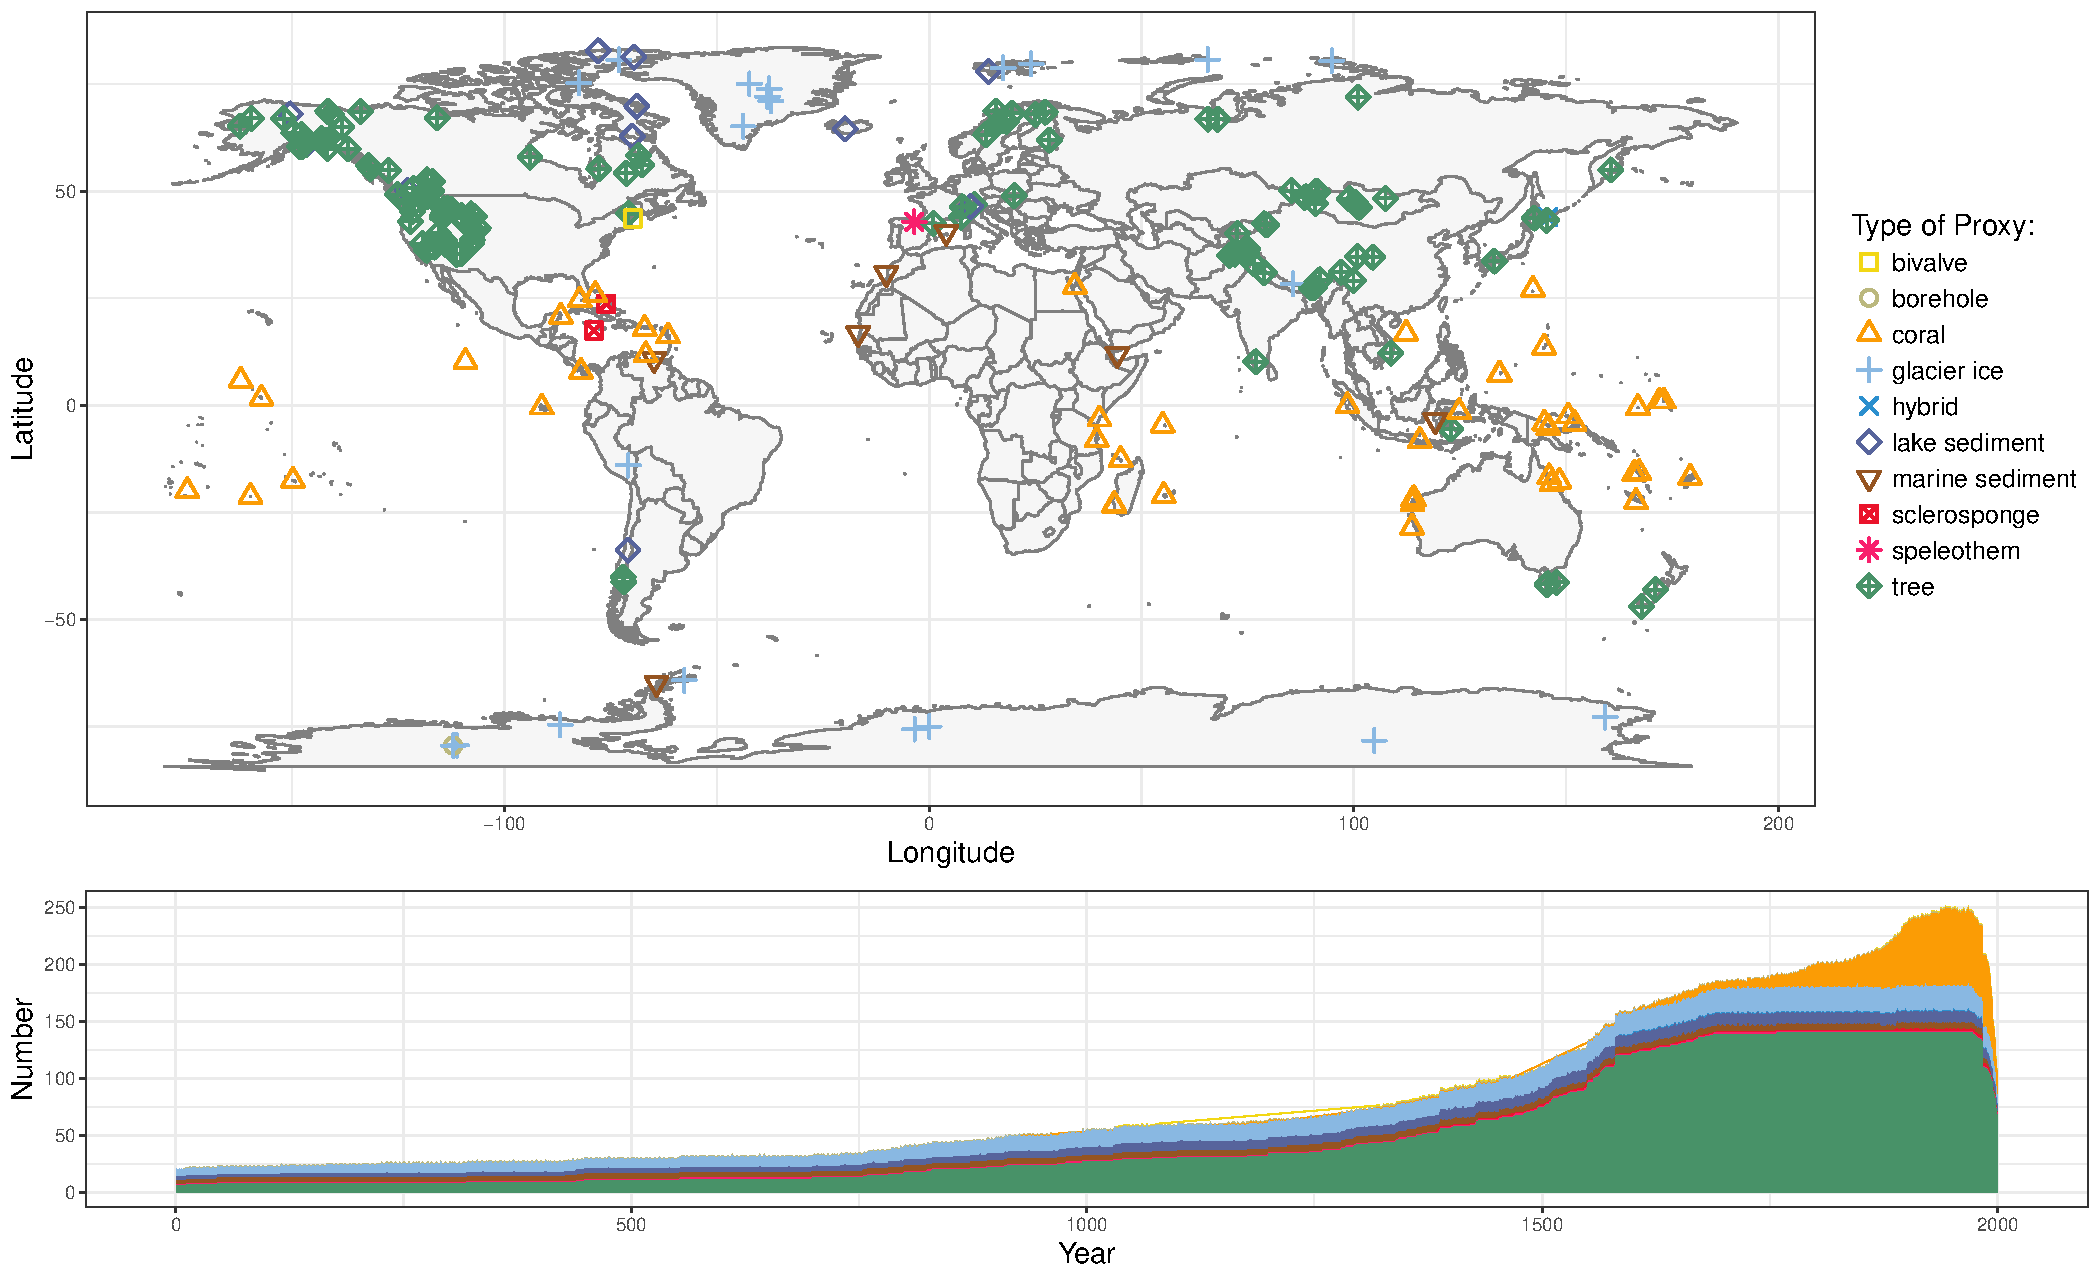
\includegraphics[scale=0.45]{CombinedMap_Area}
  \caption{Pages2k proxy distribution and temporal availability of proxies by
    type, after the screening procedure of \cite{Emile-Geay2015}.}
  \label{fig:proxy}
\end{figure}
As mentioned, proxies have different temporal horizons, as it can be shown in the
second panel of Figure~\ref{fig:proxy}. Unlike previous studies (for example \cite{Barboza2014}), in this article we try to take into account the information available in most proxies, despite their temporal diversity.


\subsection{Temperature data.}
We used the HadCRUT4 global temperature dataset provided by the Met Office Hadley
Centre and the Climatic Research Unit at the University of East Anglia, UK (version 4.4.0.0). The
data consists of historical information of temperature anomalies relative to the
period 1961-1990 in degrees Celsius, on an annual basis and calculated as
medians of spatial information (more details in \cite{Morice2012}).

\subsection{Forcing data.}
The forcing data consists of (see Figure \ref{fig:forcings} in the Appendix):
\begin{itemize}
\item Historical Greenhouse-Gases concentrations: hemispheric means of mole
  fraction of carbon dioxide in air (ppm) with annual
  resolution, taken from Coupled Model Intercomparison Project (CMIP6) (see
  \cite{Meinshausen2016}).
  
\item Volcanic forcing from Easy Volcanic Aerosol (EVA) dataset (evolv2k): (see
  \cite{Toohey2016}) reconstructed zonal mean AOD (mid-visible, i.e., 550 nm), covering the
  500 BCE to 1900 CE time period. For 1900 (or 1850) to present, \cite{Thomason2016} is
  used to fill in the forcing table, the volcanic data at varying locations is
  weighted by cosine of their corresponding latitudes.
  
\item The solar forcing data is computed from SATIRE-H
  (Holocene) at \cite{Vieira2011}. Irradiance from SATIRE-H (Holocene) is
  recorded on a decadal basis from 9495BC - 1939AD and then on a daily basis
  from 1940AD onwards. Hence, the data prior to 1939AD was interpolated using splines and after 1940AD, an annual mean is computed. For consistence of resolution of the data, annual data from 1640AD to 2000AD is also spline interpolated.
\end{itemize}
\textbf{Julien: Can you please include more details on this section?}
\section{Hierarchical Bayesian Model.}
\label{sec:model}

\subsection{Reduced Proxy.}
\label{sec:rp}
Following \cite{Barboza2014}, we reduce the dimension of the proxy dataset
through the notion of a Reduced Proxy ($RP$). First of all, we centered and
scaled the proxy variables. Then we remove proxy series whose proportion of lost
annual 
observations is larger than 5\%. Due to the diversity of start
dates in the proxies database (see Figure \ref{fig:proxy}), we divide
proxies into non-homogeneous groups where each group has dates of origin within an
interval of 250 years. As the reconstruction is taking place over a 2000 year
horizon, this creates 8 groups with the distribution shown in Table \ref{tab:distdate}.
\begin{table}
  \centering
  \begin{tabular}{c|c|c}
    \toprule
    Group & Interval (year AD) & Number \\
    \midrule
    1 & 1-250 & 19 \\
    2 & 251-500 & 25 \\
    3 & 501-750 & 29 \\
    4 & 751-1000 & 33 \\
    5 & 1001-1250 & 54 \\
    6 & 1251-1500 & 65 \\
    7 & 1501-1750 & 105 \\
    8 & 1751-2000 & 146 \\
    \bottomrule
  \end{tabular}
  \caption{Distribution of proxies according to date of origin.}
  \label{tab:distdate}
\end{table}
Two important aspects that we can notice from the distribution of Table
\ref{tab:distdate} are: (1) in the last two intervals the number of proxies is greater than
the number of available observations in the calibration period defined as
1916-2000CE (85 observations) and (2) the number of proxies is very close to the
number of available observations, which can cause overfitting issues or
dimensionality problems in the use of classical linear models. Due to the above
reasons we adjusted a multiple linear regression model between the anomalies
observed and the proxies chosen in groups 1 to 5 as covariates, all during the calibration
period. For the rest of the groups we used four different popular reduction
techniques with the aim of adjusting a linear model between the same variables over the same period: 
\begin{description}
\item[Lasso Regression (LR)]
We used a 10-fold Lasso regression where the smoothing parameter was selected
through a cross validation criteria (see \cite{Tibshirani1996} and \cite{Friedman2010} for more details). % In this case, the Lasso
% regression was fitted using the temperature anomalies observed within the
% calibration period as the dependent
% variable and the corresponding standardized proxies in each of the groups
% defined in Table \ref{tab:distdate} as covariates.
 The Lasso regression penalizes the usual sum of squares with an argument
 containing the sum of the absolute values of each coefficient in the classical
 linear regression model, multiplied by an additional parameter (see \cite{Tibshirani1996}). Due
 to the geometric nature of the term of penalization, the search of estimators
 tends to assign values very close to zero to variables that have almost null
 effects with respect to the dependent variable. Clearly, this is its main advantage
 over other methods.
% In this case, the Lasso
% regression was fitted using the temperature anomalies observed within the
% calibration period as the dependent
% variable and the corresponding standardized proxies in each of the groups
% defined in Table \ref{tab:distdate} as covariates. 
\item[Sparse Partial Least Squares (sPLS)] 
  This method has the advantage to include sparseness in the partial least squares
  estimators, in order to avoid inconsistency problems when there are a
  considerable number of noisy covariates (see \cite{Chun2010} and \cite{Chung2013}). The
  thresholding parameter is found using a 10-fold cross-validation criteria.    
\item[Sliced Inverse Regression (SIR) with CSS selection method]
  This procedure allows us to select reduced models which are similar to the
  complete model in terms of the linear correlation among SIR-QZ indices (see
  \cite{Coudret2014} and \cite{Coudret2017}). In general, the SIR methods (\cite{Li1991},
  \cite{Duan1991}, \cite{Zhong2005}, \cite{Li2008}, \cite{Coudret2014}, \cite{Weisberg2002} among
  others) reduce the dimension excess in non-parametric problems through the
  estimation of the linear space spanned by the coefficients of the covariables.
  In our case, we opt to use 8 slices and 4,6 and 2 EDR directions to approximate the linear
  subspace of the 6th, 7th and 8th set of proxies respectively. Finally we studied the association between proxies and temperatures
  through a linear regression among the corresponding directions and the anomalies observed
  during the calibration period. 
\item[Principal Component Regression (PCR)]
We computed the first 5 principal components on each set of proxies and we fitted a
regression model between the temperature in the calibration period and the PCs
as covariates. This type of methodology has been frequently criticized (see
\cite{Jolliffe1982} and \cite{Tibshirani1996}),
but we consider it as a benchmark for the first three methods. 
\end{description}
Finally, we computed the reduced proxies by predicting the anomalies in the
reconstruction period under any of the above methods and any of the groups in
Table \ref{tab:distdate}. The eight reduced proxies for each methodology are
shown in the upper panel of Figure \ref{fig:RPs} in the Appendix. Also note that
the obtained reduced proxies are highly correlated among methods, see lower
panel of Figure \ref{fig:RPs}.  

\subsection{Model Specification}
\label{sec:model}

Our models are based on the one presented in \cite{Barboza2014}. Now we define
some notation, assuming that all the variables are set at time $t$.
\begin{itemize}
\item $RP_t^i$: $i$-th reduced proxy at time $t$.
  
\item $T_t$: temperature anomaly at time $t$.
  
\item $\tilde C_t = \log (C_t)$. Transformed greenhouse gases. The log
  transformation is chosen to approximate the radiative forcing due to changes
  in the equivalent CO$_2$ concentration. (see \cite{Barboza2014})
  
\item $\tilde V_t = \log (-V_t+1)$. Transformed volcanic forcing. More details
  on the choice of the transformation in \cite{Barboza2014}.
  
\item $B_t^{k,\tau}$. $k$-th B-Spline basis function at time $t$ with knot
  sequence $\tau$ (more details in \cite{DeBoor2001} and \cite{Ramsay2005}). We assume that the
  B-Spline basis is composed by cubic polynomials.  
\end{itemize}
With the above notation we can define two types of model as extensions of the
one defined in \cite{Barboza2014}, taking advantage of more reduced proxies:
\begin{description}
\item[State-Space model without forcings (Model SSnF)]
Basically, we would be defining a data level (according to the hierarchical bayesian models' jargon)
  for each available $RP$:
\begin{align}\label{eq:ssnf}
  \begin{cases}
    RP_t^i&=\alpha_0^i+\alpha_1^iT_t+\epsilon^i_t\\
  T_t&=\beta_0+\sum_{k=1}^{K(\tau)}\beta_k B_t^{k,\tau}+\eta_t
  \end{cases}
\end{align}
where $\{\alpha^i_j\}$ and $\{\beta_k\}$ are random parameters for
$i=1,\ldots,N$, $j=0,1$ and $k=1,\ldots,K(\tau)$. The number of reduced proxies is
$N\geq 1$. For simplicity, the error terms
$\epsilon^i_t$ and $\eta_t$ are assumed to be
independent normally-distributed random variables with finite variances
$\{\sigma^2_{\epsilon^i}\}$ and $\sigma^2_{\eta}$ respectively. These variances
are also considered as random and do not depend on time $t$. The main idea of
this model is to evaluate the central hypothesis of this article, that is, the
paleoclimate reconstruction can be performed without taking into account the
external forcings, as long as they are replaced with deterministic
functions that allow to describe the mean behavior of the series of anomalies.
\item[State-Space model with forcings (Model SSwF)]
As a second model we substitute the mean function in the second equation of
\eqref{eq:ssnf} with a linear combination of the external forcings:    
\begin{align}\label{eq:sswf}
  \begin{cases}
    RP_t^i&=\alpha_0^i+\alpha_1^iT_t+\epsilon^i_t\\
  T_t&=\beta_0+\beta_1S_t+\beta_2\tilde V_t+\beta_3\tilde C_t+\eta_t
  \end{cases}
\end{align}
\end{description}
The models \eqref{eq:ssnf} and \eqref{eq:sswf} are defined for
$t=1,\cdots,2000$ (Common Era). It is also important to add that we focus on
models with independent error structures since in \cite{Barboza2014} the authors
found that the greatest impact on the predictive capacity of these hierarchical
models is obtained when the forcings are added and not so much when the error
structures are more complex.

\section{Results.}
\label{sec:results}

The models proposed in equations \eqref{eq:ssnf} and \eqref{eq:sswf} were
implemented using the R package \textbf{r-inla}\footnote{www.r-inla.org}. The
implementation was based on the recommendations of \cite{Ruiz-Cardenas2012} and
\cite{Muff2015} on the use of the INLA methodology in state-space models,
dynamic linear models and, in general, measurement error models. These
recommendations together with \cite{Martins2013} allow
great flexibility when we work with bayesian models with several levels of
information, in particular in the case of levels of hierarchical models.

Like any hierarchical bayesian model, the most basic level of information
corresponds to the level of prior information. This is defined through the
following hypothesis:
\begin{itemize}
\item $\alpha^i_j\sim N(0,3)$, $\beta_\ell \sim N(0,3)$ for $i=1,\ldots,N$, $j=0,1$ and $\ell=0,\ldots,3$
  (Model SSwF) or $\ell=0,\ldots,K(\tau)$ (Model SSnF). The choice of the variance is
  completely arbitrary, but the main idea is to select a relatively large one.
  
\item $\rho_i := -\log \sigma^2_{\epsilon^i}\sim \text{log-gamma}(1,10^{-20})$
  (very small precision) for $i=1,\ldots,N$.
  
\item $\rho_0 := -\log \sigma^2_\eta \sim \text{log-gamma}(1,10^{-20})$ (very
  small precision).
\end{itemize}

As a first exercise, we analyze the change in the predictive capacity of the
reconstruction model when more equations involving proxies are included. We used
two scoring rules in \cite{Gneiting2007a} as measures of predictive ability:
IS$_\alpha$ (Interval Score at $\alpha$ level) and CRPS (Continuous Ranked
Probability Score). These scores have been previously employed in the
verification of point forecasts in environmental sciences for example, as well as the area
of paleoclimatic reconstructions (see \cite{Barboza2014} and
\cite{Scheuerer2014}). Table \ref{tab:comparisontot} contains the predictive
measures using the observed anomalies and INLA's prediction intervals over the
testing period 1914-2000. We compared in this case Model SSwF with a single RP
(the longest available) with respect to model SSwF using the 8 available reduced
proxies, where the latter are calculated under the four dimension reduction
methods explained above.


\begin{table}
  \centering
\begin{tabular}{lll|rrr}
  \toprule
 \textbf{Model} & $N$ & \textbf{Method} & IS$_{80}$ & IS$_{95}$ & CRPS \\ 
  \midrule
  SSwF & 1 & - & 0.5249 & 0.1988 & 0.2278 \\
  \midrule
  SSwF & 8 & PCR & 0.1622 & 0.0542 & 0.0702 \\ 
  SSwF & 8 & LASSO & 0.2465 & 0.1180 & 0.0864 \\ 
  SSwF & 8 & SPLS & 0.1755 & 0.0586 & 0.0687 \\ 
  SSwF & 8 & SIR & 0.2439 & 0.1144 & 0.0891 \\
  \midrule
  SSnF & 8 & PCR & 0.1583 & 0.0532 & 0.0435 \\ 
  SSnF & 8 & LASSO & 0.1881 & 0.0640 & 0.0697 \\ 
  SSnF & 8 & SPLS & 0.1819 & 0.0611 & 0.0574 \\ 
  SSnF & 8 & SIR & 0.1649 & 0.0550 & 0.0462 \\ 
   \bottomrule
\end{tabular}
  \caption{Comparison of predictive measures.}
  \label{tab:comparisontot}
\end{table}


% \begin{table}
%   \centering
%   \begin{tabular}{c|rrr}
%     \toprule
%     Number of RPs-Method& IS$_{80}$ & IS$_{95}$ & CRPS \\ 
%     \midrule
%     1 RP & 0.5249 & 0.1988 & 0.2278 \\ 
%     8 RPs-PCR & 0.1622 & 0.0542 & 0.0702 \\ 
%     8 RPs-LASSO & 0.2465 & 0.1180 & 0.0864 \\ 
%     8 RPs-SPLS & 0.1755 & 0.0586 & 0.0687 \\ 
%     8 RPs-SIR & 0.2439 & 0.1144 & 0.0891 \\ 
%     \bottomrule
% \end{tabular}
%   \caption{Comparison of predictive measures in Model 1.}
%   \label{tab:comparison1}
% \end{table}
It is evident that there is a substantial improvement
in all the measures when we use all the available reduced proxies under any
method. Also note that, among the models with external forcings, the techniques that
guarantees better results in terms of prediction are PCR and SPLS.

We are also interested in verifying whether a linear combination of B-splines
models the average behavior of the anomalies without the inclusion of external
forcings at all. It is clear from equation \eqref{eq:ssnf} that one of the
drawbacks of Model 2 is the arbitrariness of $K(\tau)$. Therefore, for each of
the methods in section 4.1, the IS and CRPS measures were calculated for a fixed
value of $K(\tau)$ over a grid defined in [1,50]. After this, the best $K(\tau)$
for each method was selected using the IS and CRPS measures. These results are
shown in the last four lines in Table \ref{tab:comparisontot}. Due to the comments of the above paragraph, we opt to
use all the reduced proxies in this case.
% \begin{table}
%   \centering
%   \begin{tabular}{c|rrr}
%   \toprule
% Method  & IS$_{80}$ & IS$_{95}$ & CRPS \\ 
%   \midrule
% PCR & 0.1583 & 0.0532 & 0.0435 \\ 
%   LASSO & 0.1881 & 0.0640 & 0.0697 \\ 
%   SPLS & 0.1819 & 0.0611 & 0.0574 \\ 
%   SIR & 0.1649 & 0.0550 & 0.0462 \\ 
%    \bottomrule
% \end{tabular}
%   \caption{Comparison of predictive measures of Model 2.}
%   \label{tab:comparison2}
% \end{table}
Note that PCR method attains a better performance in terms of all the three
predictive measures than the
rest of the methods, even though SIR differs very little in its corresponding
measures. 

Based on the above, we consider that Model SSnF's reconstructions based on PCR and SIR
with $K(\tau)$ = 29 and $K(\tau)$ = 24 respectively represent the best results
especially for the CRPS measure. Due to the criticism in the PCR methodology
(see \cite{Jolliffe1982} and \cite{Tibshirani1996}), we point out the convenience of using SIR as the best methodology for
Model SSnF. However, the graphical results between both cases are very similar as
can be seen in the following figures. First note that the reconstructions of the
temperature anomalies in the Common Era are shown in
Figure \ref{fig:paleoCE1}. Both
show a similar behavior, in terms of trend and dispersion. The same can be said
for a closer look of the reconstructions during the period 1900-2000 (see
Figure \ref{fig:paleo19001}). For comparison purposes,
we also include the reconstructions of Model SSwF with the PCR method (see the
upper panels of 
figures \ref{fig:paleoCE4} and \ref{fig:paleo19004} in the appendix), where the
main difference corresponds to the period 1-250 in terms of the variance of the
mean function, mainly due to the sensitivity of the B-Spline basis to
discrepancies among reduced proxies in a fixed time period. Also note that the
resulting posterior densities of the external forcings (see Figure
\ref{fig:betas} in the Appendix) suggest that both $S_t$
and $\tilde C_t$ are quite significant to explain the temperature anomalies.    
\begin{figure}
  \centering
  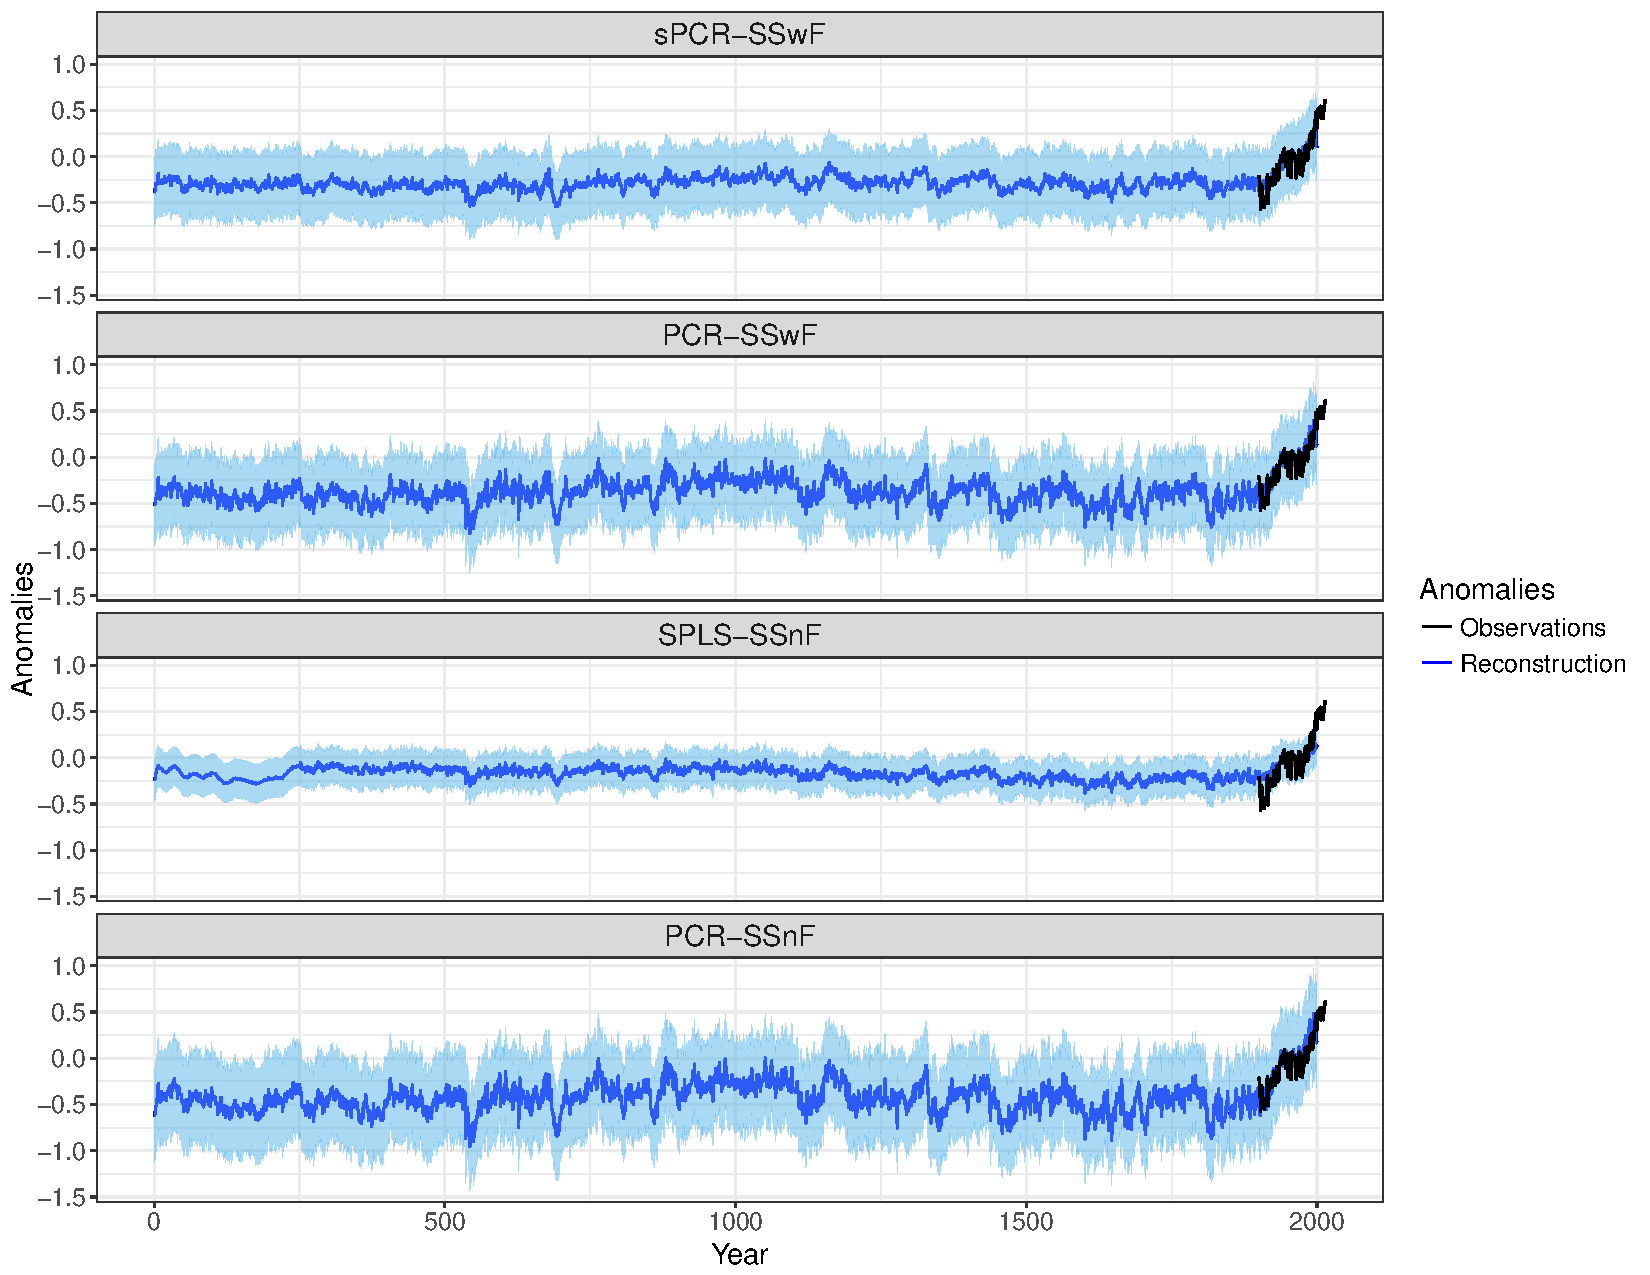
\includegraphics[scale=0.45]{RecCE_Final}
  \caption{Paleoclimate Reconstruction in the Common Era (CE) with 95\%
    prediction bands. Model SSnF.}
  \label{fig:paleoCE1}
\end{figure}

\begin{figure}
  \centering
  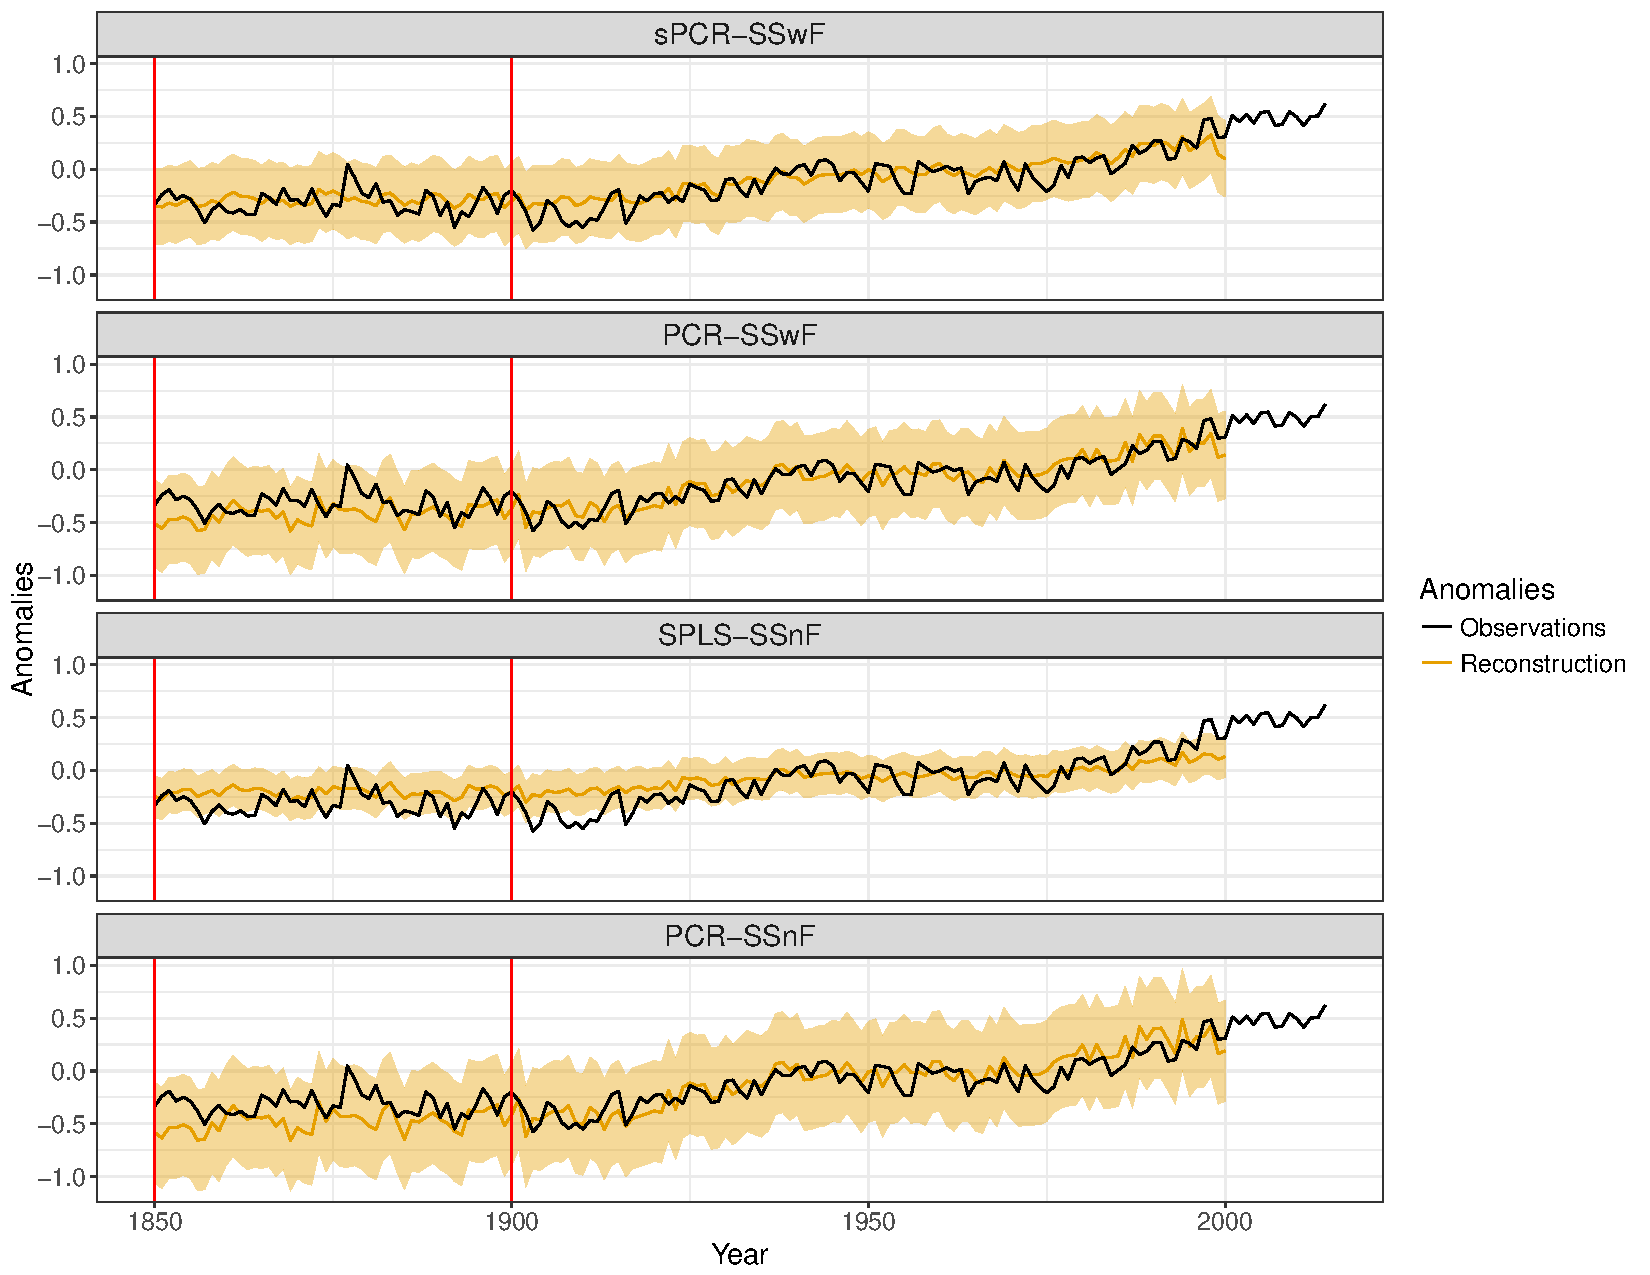
\includegraphics[scale=0.45]{Rec1900_Final}
  \caption{Paleoclimate Reconstruction 1900-2000 with 95\%
    prediction bands. Model SSnF.}
  \label{fig:paleo19001}
\end{figure}

Finally, we also compare the nature of the linear function that determines the
mean behavior of the state equation in both models. As the coefficients that
accompany the covariates are random (External forcings for Model SSwF, B-Splines
for Model SSnF) then it is possible to calculate confidence bands for the mean
function in both cases. This is illustrated in Figure \ref{fig:meanfunction}.
\begin{figure}
  \centering
  \includegraphics[scale=0.4]{MeanFunction_comp}
  \caption{Mean function of the state equation and its 95\% confidence band.}
  \label{fig:meanfunction}
\end{figure}
Note that the variance and the stability of the mean function are much greater
in the best case of Model SSnF than in the best case of Model SSwF. This could be an
indicator that Model SSwF has a greater bias in its mean behavior, which is a
negative aspect in the reconstruction as a whole.

The computational efficiency of the INLA procedure is quite remarkable, not only
for our case but in most of the previous works on the topic (see \cite{Rue2009},
\cite{Blangiardo2013}, \cite{Ruiz-Cardenas2012} for a few examples). The
computational time of an MCMC method applied on Model SSwF with 1 RP (simplest
model) was
aproximately 14 hours, whereas the computational time of INLA on Model SSwF with
8 RPs (most complex model) was aproximately 11 minutes \footnote{This comparison
was performed on an Ubuntu 16.04 server with Intel Xeon E5-2630 (8-cores,
2.40GHz) and 64 GB of RAM.}. A graphical comparison of the reconstructions using
both methods is shown in Figures \ref{fig:paleoCE4} and \ref{fig:paleo19004} in
the Appendix. Note that the MCMC reconstruction is cooler than INLA's, due
mainly to the inclusion of more information from the remaining 7 reduced
proxies. The MCMC confidence bands along the reconstruction period are narrower,
this together with the information observed in Figure \ref{fig:meanfunction}
suggest that the reconstruction obtained through a MCMC technique has larger
bias than the one obtained with INLA method.


\section{Conclusions.}
\label{sec:conclusions}

%\printbibliography

\bibliographystyle{plain}
\bibliography{biblioteca}


\newpage
\appendix

\section{Additional Plots}
\begin{figure}[H]
  \centering
 \includegraphics[scale=0.4]{RPs_typeandCor} 
  \caption{Reduced Proxies and Correlation Matrices among methods.}
  \label{fig:RPs}
\end{figure}

% \begin{figure}[H]
%   \centering
%   \includegraphics[scale=0.4]{PAGES_composites_PCR5} 
%   \caption{Reduced Proxies using PC regression.}
%   \label{fig:proxiespcr}
% \end{figure}

\begin{figure}[H]
  \centering
  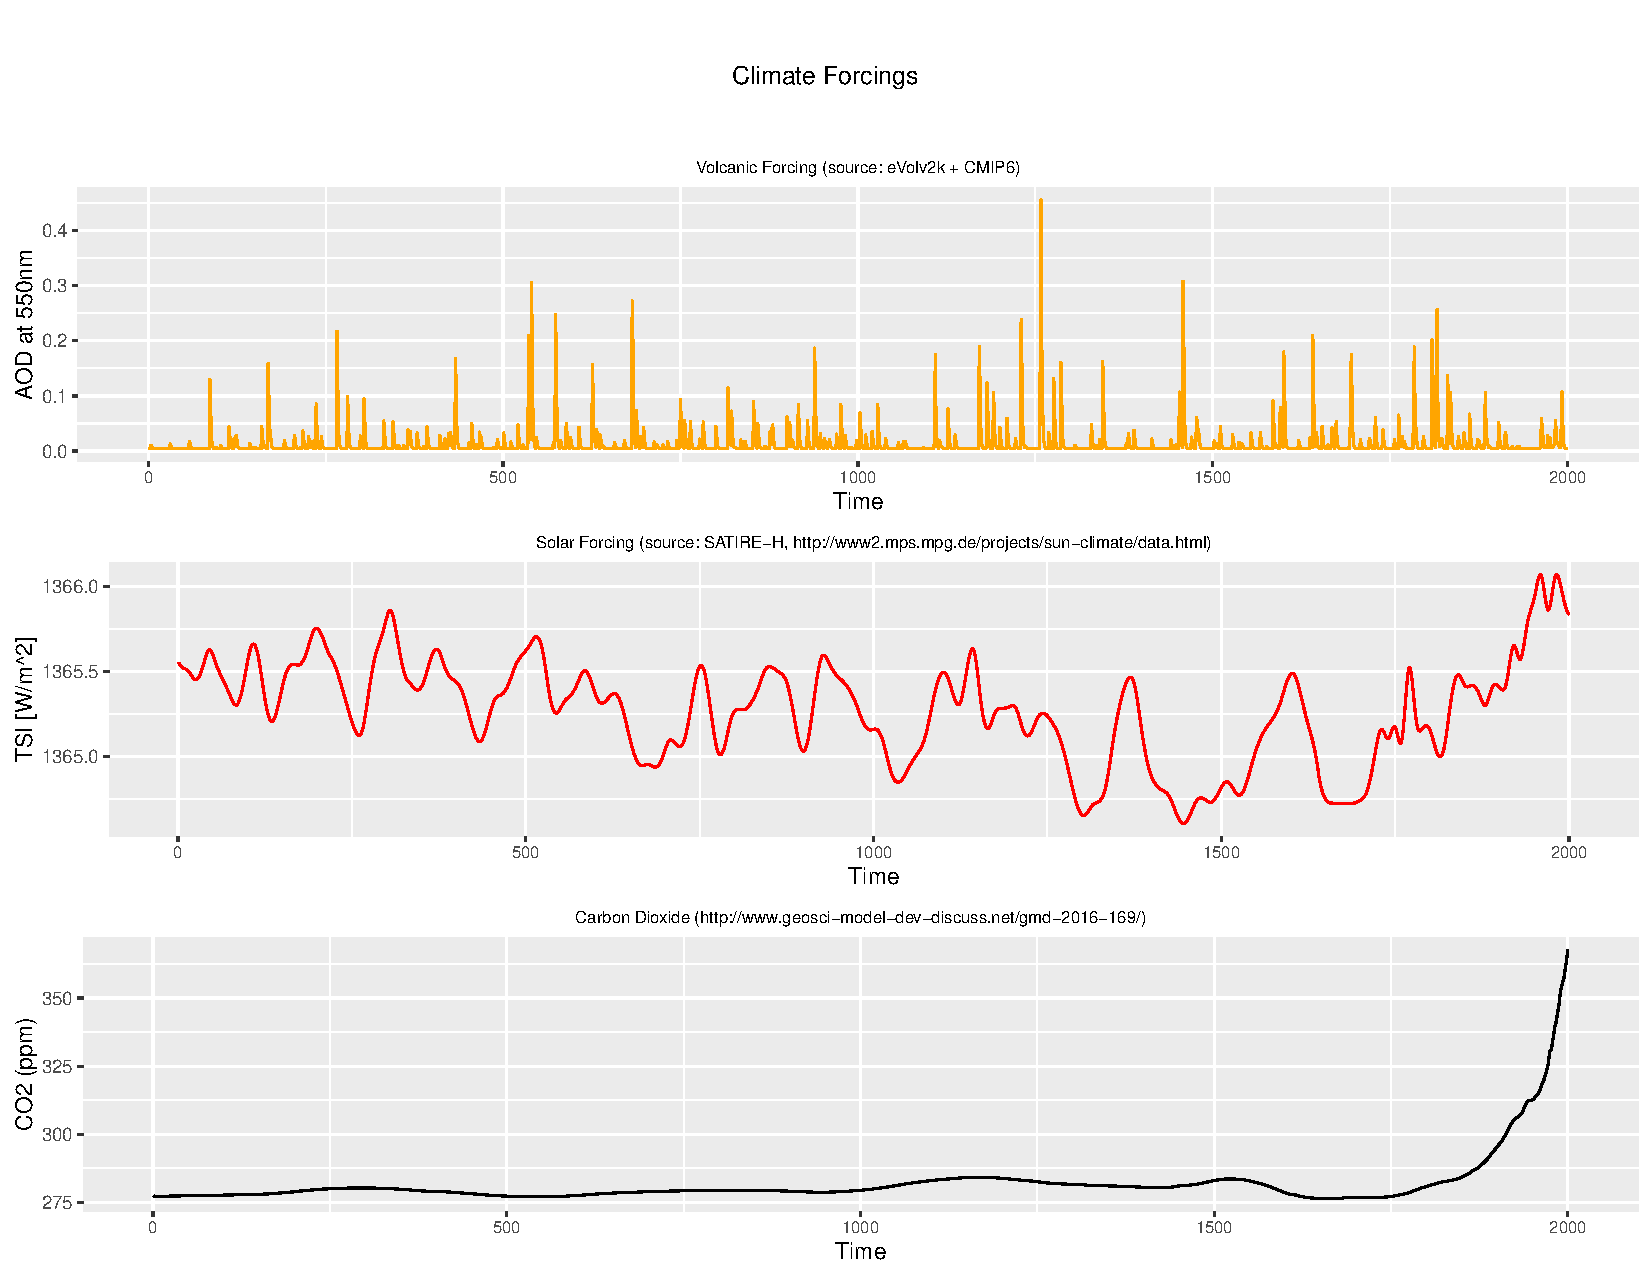
\includegraphics[scale=0.35]{forcings}
  \caption{Climate Forcings in the Common Era (1-2000 AD)}
  \label{fig:forcings}
\end{figure}

% \begin{figure}[H]
%   \centering
%   \includegraphics[scale=0.35]{RecCE_PCR_Splines}
%   \caption{Paleoclimate Reconstruction in the Common Era (CE) with 95\%
%     prediction bands. PCR Method - Model 2.}
%   \label{fig:paleoCE3}
% \end{figure}

% \begin{figure}[H]
%   \centering
%   \includegraphics[scale=0.4]{Rec1900_PCR_Splines}
%   \caption{Paleoclimate Reconstruction 1900-2000 with 95\%
%     prediction bands. PCR Method - Model 2.}
%   \label{fig:paleo19003}
% \end{figure}

\begin{figure}[H]
  \centering
  \includegraphics[scale=0.35]{RecCE_Forcings}
  \caption{Paleoclimate Reconstruction in the Common Era (CE) with 95\%
    prediction bands. Model SSwF (PCR) under two methods: INLA and MCMC.}
  \label{fig:paleoCE4}
\end{figure}

\begin{figure}[H]
  \centering
  \includegraphics[scale=0.35]{Rec1900_Forcings}
  \caption{Paleoclimate Reconstruction 1900-2000 with 95\%
    prediction bands. Model SSwF (PCR) under two methods: INLA and MCMC.}
  \label{fig:paleo19004}
\end{figure}


\begin{figure}[H]
  \centering
  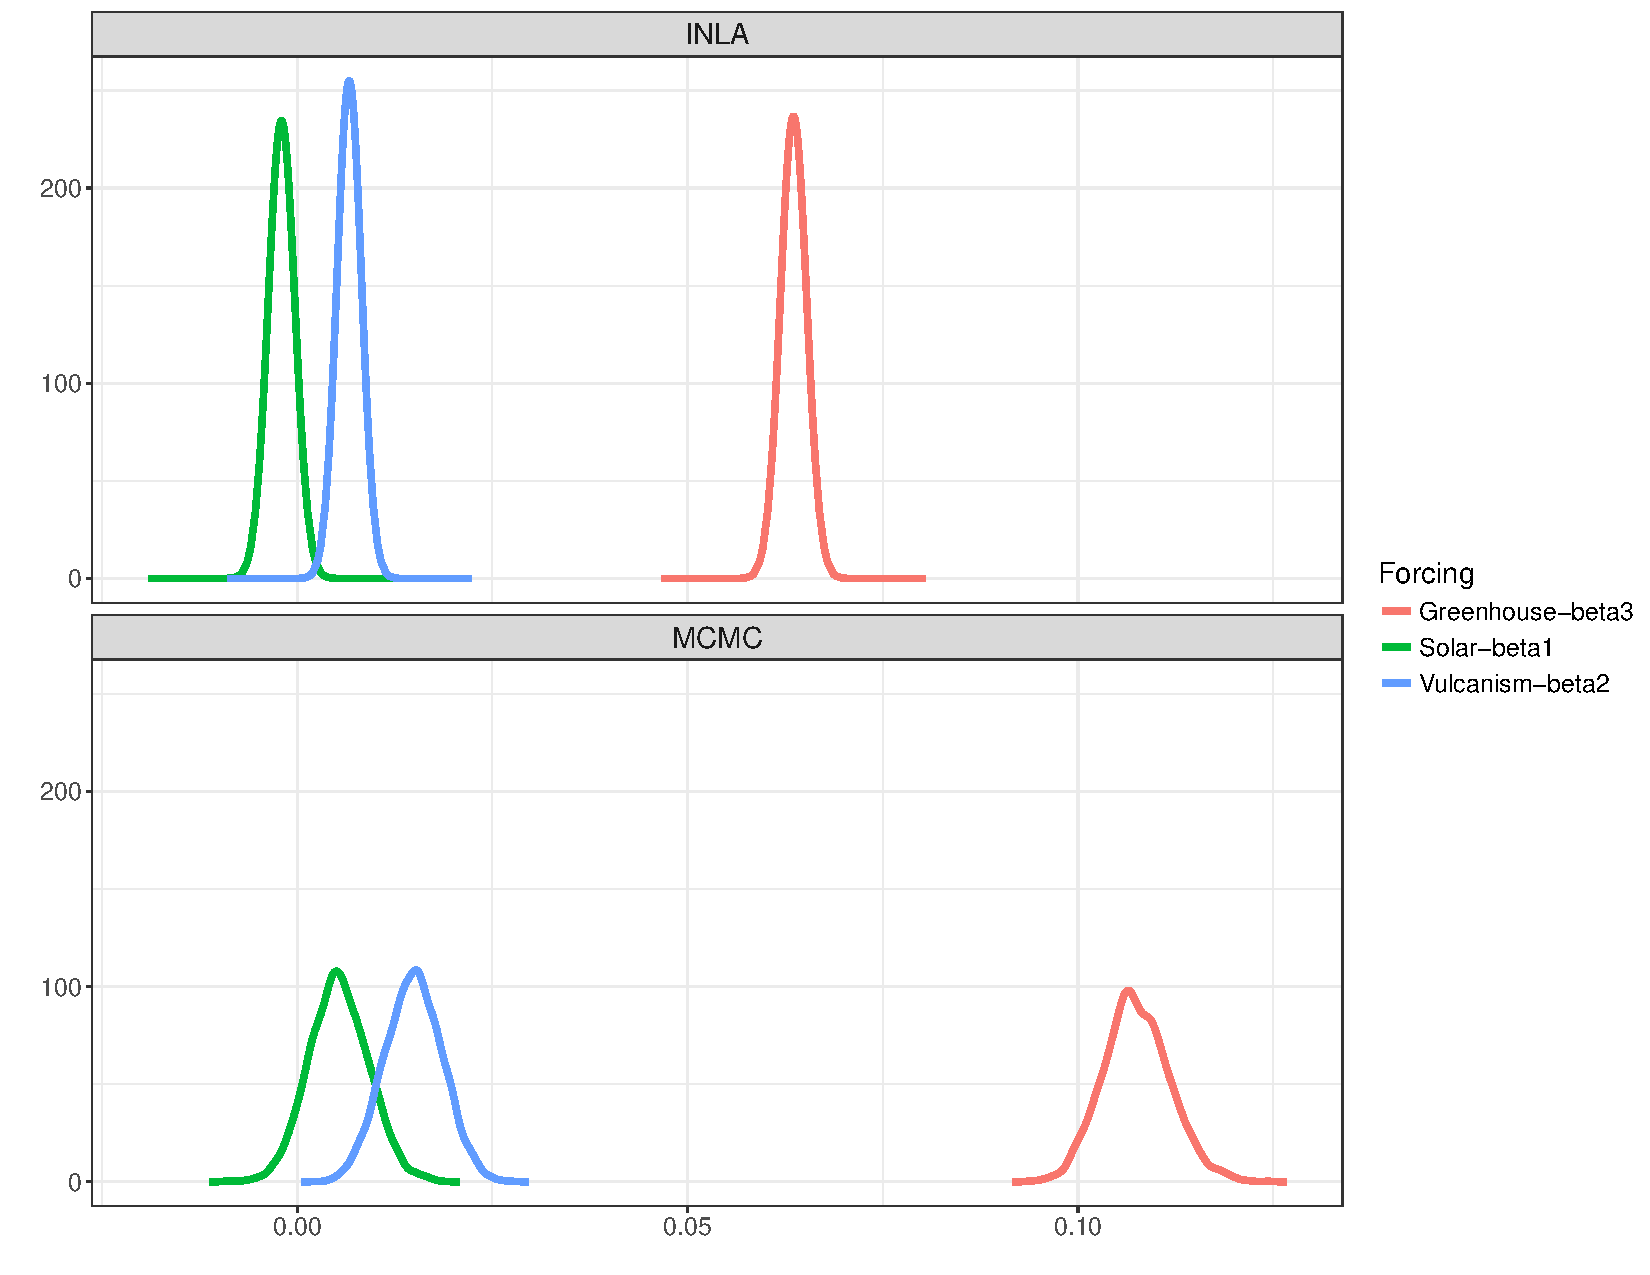
\includegraphics[scale=0.4]{PlotBetas}
  \caption{Posterior densities of $\beta_1$, $\beta_2$ and $\beta_3$ for Model SSwF
  (PCR)}
  \label{fig:betas}
\end{figure}

\end{document}
